\documentclass[UTF8]{ctexart}
\usepackage{bookmark}
\usepackage{hyperref}
\usepackage{geometry}
\geometry{a4paper,scale=0.8}
\usepackage{ctex}
\usepackage[style=caspervector,backend=biber,utf8]{biblatex}
\addbibresource{reference.bib}
\usepackage{booktabs}
\usepackage{array}
\usepackage{fancyhdr}
\pagestyle{fancy}
\fancyhf{}
\renewcommand\footrulewidth{1pt}
\lhead{王铠泽}
\rhead{PB18020766}
\chead{\href{mailto:volar@mail.ustc.edu.cn}{volar@mail.ustc.edu.cn}}
\rfoot{中国科学技术大学}
\lfoot{\today}
\usepackage{graphicx}
\usepackage{float}
\usepackage{subfigure}


\begin{document}

	\centering\textbf{\LARGE{计算物理A第二次作业}}
	
	
	王铠泽\qquad PB18020766
	
		
	\section{作业题目}
	
	\begin{itemize}
		\item 用16807产生器测试随机数序列中满足关系 $X_{n-1}<X_{n+1}<X_n$
		的比重。讨论Fibonacci延迟产生器中出现这种关系的比重。
	\end{itemize}
	
	\section{实现方法}
	
	\begin{itemize}
		\item Lehmer线性同余随机数产生器
		
		$$I_{n+1}=(aI_n+b)\,mod\,m$$
		$$x_n=I_n/m$$
		在本次实验中,主要采用的是16807产生器(最低标准产生器),即 $a=16807,b=0,m=2^{31}-1$
		\item Schrage方法
		
		为了在计算过程中中间数据不溢出,使用$Shrage$方法来求取余数。
		
		$$az\,mod\, m=\left\{
		\begin{array}{lcl}
		a(z\,mod\,q)-r[z/q]       &      &a(z\,mod\,q)-r[z/q] \geq0 \\
		a(z\,mod\,q)-r[z/q]+m&      & otherwise
		\end{array} \right. $$
		
		\item Fibonacci产生器
		
		这是一种延迟产生器,首先种下$max\{p,q\}$个种子,然后根据如下公式迭代产生随机序列:
		$$I_n=I_{n-p}\otimes I_{n-q}$$
		其中$\otimes$可以代表加法,减法或者XOR运算等。
		本次实验中,采用16807产生器和其默认种子$I_0=1$产生$Fibonaci$产生器的前$max\{p,q\}$个数据,运算符采用加法运算符。
		
		实验中,$(p,q)$取如下建议的经验值:
		$(24,55),(38,89),(37,100),(30,127)$
		
	\end{itemize}
	\section{程式说明}
	
	\begin{itemize}
		\item Fibonacci.c 
		
		该程式分别通过16807产生器和不同$(p,q)$组合下$Fibonacci$产生器产生100000个随机数并且统计题目要求关系比例。
		
		包含以下函数:
		\subitem int shrage (int a, int m, int In)
		
		返回值是 $aI_n\,mod\,m$
		
		\subitem int initial (int n)
		
		$n=0$ 为16807产生器默认种子 $I_0=1$, $n=1$ 为时间种子生成 $I_0$。本实验中采用默认种子。
		
		\subitem int main()
		
		main函数分为三个模块,分别是用16807产生器生成随机数,用不同$(p,q)$组合的$Fibonacci$产生器生成随机数,计算比例。
		
		\item ratio.txt
		
		该文本文件记录了16807产生器和不同的$Fibonacci$产生器对应的关系比例。	
	\end{itemize}
	
	\section{计算结果}
\begin{flushleft}
		在理想条件下,得到$X_{n-1}<X_{n+1}<X_n$等价于在$[0,1]\times[0,1]\times[0,1]$区域上找到$x<z<y$区域的概率。其体积为一个四棱锥,为 $\frac{1}{2}\times\frac{1}{3}=\frac{1}{6}$。如下图所示区域即为所求。
\end{flushleft}
	
	\begin{figure}[H]
	\centering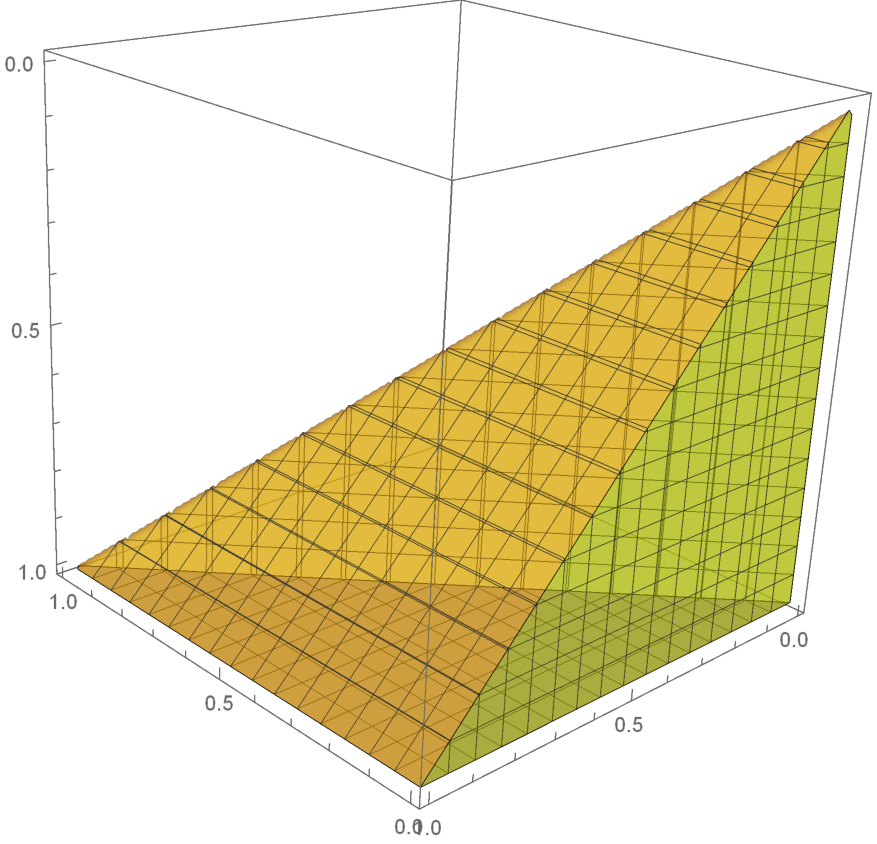
\includegraphics[width=3in]{ideal.pdf}
	\caption{理想期望值}\label{fig:1}
	\end{figure}
	\subsection{比例关系比较}
\begin{table}[H]
	\centering
	\setlength{\tabcolsep}{10mm}{
		\begin{tabular}{@{}lll@{}}
			\toprule
			产生器&$X_{n-1}<X_{n+1}<X_n$比例&和理想比例之差绝对值 \\ \midrule
			16807&0.165300&0.001367\\
			$Fibonacci,(p,q)=(55,24)$&0.165980&0.000687\\
			$Fibonacci,(p,q)=(89,38)$&0.165700&0.000967\\
			$Fibonacci,(p,q)=(100,37)$&0.165840&0.000827 \\ 
			$Fibonacci,(p,q)=(127,30)$&0.168300& 0.001633\\ 
			$Fibonacci,(p,q)=(250,103)$&0.166190& 0.000477\\
			$Fibonacci,(p,q)=(31,3)$&0.168060&0.001393\\ \bottomrule
			
	\end{tabular}}
	\caption{不同产生器$X_{n-1}<X_{n+1}<X_n$比例}
\end{table}
	
	
	

	\section{总结}
	\begin{itemize}
		\item $Fibonacci$产生器的质量一定程度上依赖于$(p,q)$的选择。本次实验中,$(250,103)$的产生器效果最理想。而$(127,30)$效果一般。相比之下,满足准则:$p^2+q^2+1=prime\,number$的$(31,3)$效果一般。很多建议的$(p,q)$数值都不满足该准则,所以$Fibonacci$参数选择可能是一个比较复杂的经验依赖性工作。
		\item 总体上看,$Fibonacci$产生器比16807产生器效果略好。
		\item $Fibonacci$由于需要的种子数量较多,其对随机数生成的质量有影响。本次实验采用16807产生种子。
	\end{itemize}
	\clearpage
\end{document}